
\section{Невронски мрежи}

Имплементација на алгоритмот за повратна пропагација за учење на параметрите на
невронската мрежа. Овој алгоритам ќе го искористиме за препознавање на ракописно
напишани цифри. Ова е корисно во автоматско читање на поштенски кодови, чекови,
сметки и слично.

\subsection{Визуелизација на податоците}

\begin{figure}[htb]
\centering
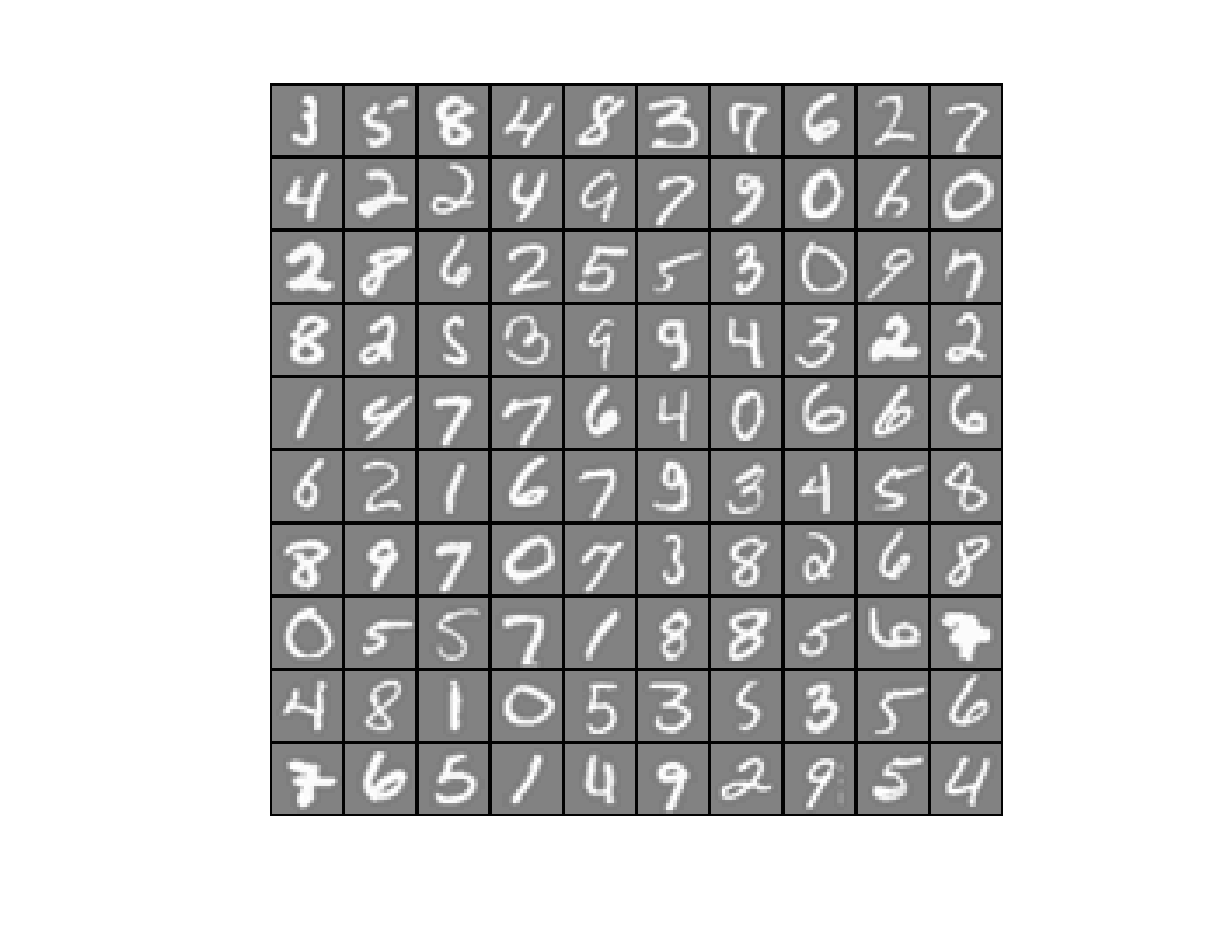
\includegraphics[width=.9\textwidth]{src/neuralNetwork2/nn}
\caption{Примероци од податочното множество}
\label{fig:neuralNetworkData}
\end{figure}

Податочното множество (дел е прикажан на слика \ref{fig:neuralNetworkData}) за овој алгоритам е
составено од 5000 тренинг примероци, од кој секој примерок е црно-бела слика од 20x20 пиксели. Секој пиксел се
репрезентира со децимален број кој го означува интензитетот. Овие 400 пиксели се
сместени во еднодимензионален вектор. Секој од овие тренинг примероци
претставува ред од матрицата X. Со ова се добива матрица од 5000 по 400 во која
секој ред е примерок за слика од ракописно напишана цифра.

\[
	X = \begin{bmatrix}
		    (x^{(1)})^T \\
			(x^{(2)})^T \\
			\vdots \\
			(x^{(m)})^T
			
		\end{bmatrix}
\]

Вториот дел од податочното множество е 5000-димензионален вектор $y$ кој 
ги содржи целните ознаки за податочното множество. За да се постигне
компатибилност со индексирањето во Octave/Matlab, каде што не постои 0 индекс,
цифрата 0 е пресликана во вредноста 10. Така, цифрата „0“ е означена како „10“,
додека цифрите од „1“ до „9“ се означени како „1“ до „9“ во нивниот природен
редослед.

\subsection{Репрезентација на моделот}

\begin{figure}[htb]
\centering
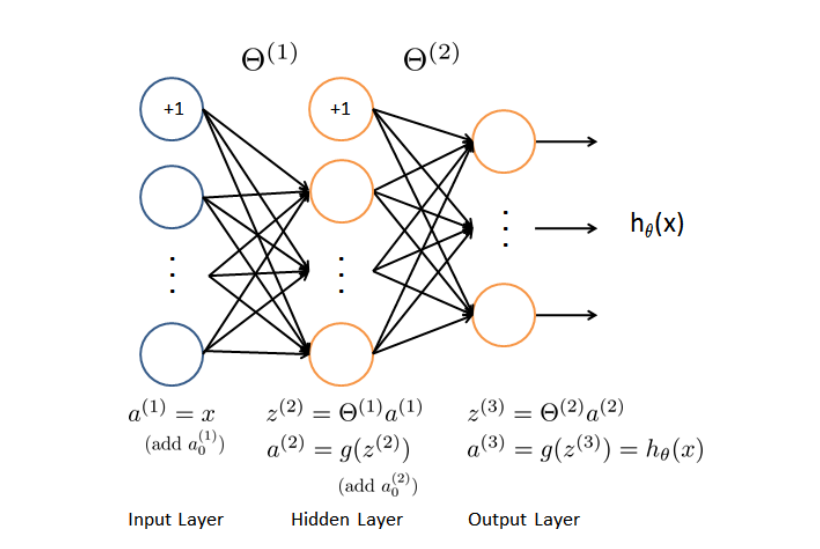
\includegraphics[width=.9\textwidth]{src/neuralNetwork2/neuralNetwork}
\caption{Моделот на невронска мрежа}
\label{fig:neuralNetwork}
\end{figure}

На слика \ref{fig:neuralNetwork} е прикажан моделот на невронската мрежа. Се
состои од 3 слоеви: влезен слој, скриен слој и излезен слој. На влезот на оваа
невронска мрежа се дигиталните слики. Затоа што секоја слика е со големина 20 x
20, влезниот слој е составен од 400 влезни единици.

\subsection{Feedforward пропагација и предикција}

Алгоритмот за feedforward пропагација ја пресметува $h_\theta(x^{(i)})$ за секој
примерок $i$ и ја враќа предвидената вредност. Слично како кај стратегијата за класификација
еден-против-сите, предвидувањето на невронската мрежа ќе биде ознаката со
најголема вредност $(h_\theta(x))_k$.

\lstinputlisting[firstline=6,lastline=17,caption=Имплементација
на функцијата predict]{src/neuralNetwork1/predict.m}


\subsection{Feedforward и cost функција}

Функцијата на чинење на невронска мрежа (без регуларизација) е

\[
	J(\theta) = \frac{1}{m}\sum_{i = 1}^{m}\sum_{k =
	1}^{K}[-y^{(i)}_k\log((h_\theta(x^{(i)}))_k) -
	(1 - y^{(i)}_k)\log(1 - (h_\theta(x^{(i)}))_k)],
\]

каде што $h_\theta(x^{(i)})$ се пресметува како на слика \ref{fig:neuralNetwork}
 и $K = 10$ е бројот на можни ознаки. Со $(h_\theta(x^{(i)}))_k = a^{(3)}_k$ се
 означува активацијата (излезната вредност) на $k-th$ излезна единица.
 Оригиналните вредности за излезната ознака $y$ се 1, 2, \ldots, 10, за
 тренирање на невронска мрежа, треба сите ознаки да се претворат во соодветни
 вектори кои ги содржат единствено вредностите 0 и 1:
 
 \[	
	y = \begin{bmatrix}
		    1 \\
			0 \\
			0 \\
			\vdots \\
			0
			
		\end{bmatrix},
		\begin{bmatrix}
		    0 \\
			1 \\
			0 \\
			\vdots \\
			0
			
		\end{bmatrix},
		\ldots
		or
		\begin{bmatrix}
		    0 \\
			0 \\
			0 \\
			\vdots \\
			1
			
		\end{bmatrix}
 \]

На пример, ако $x^{(i)}$ е слика од цифрата 5, тогаш соодветното $y^{(i)}$ (кое
треба да се искористи во функцијата на чинење) треба да биде 10-димензионален вектор
со $y_5 = 1$, а останатите елементи 0.

\lstinputlisting[firstline=17,lastline=60,caption=Имплементација
на функцијата на
чинење,basicstyle=\ttfamily\scriptsize]{src/neuralNetwork2/nnCostFunction.m}

\subsection{Backpropagation}

\subsubsection{Сигмоид градиент}

Градиентот за сигмоид функцијата се пресметува како

\[
	g'(z) = \frac{d}{dz}g(z) = g(z)(1 - g(z))
\]

каде што

\[
	sigmoid(z) = g(z) = \frac{1}{1 + e^{-z}}.
\]

\subsubsection{Случајна иницијализација}

Кога се тренираат невронски мрежи, важно е да параметрите да се иницијализираат
случајно за да се наруши симетријата. Една ефективна стратегија за случајна
иницијализација е случајно да се изберат вредности за $\theta(l)$ рамномерно во
опсегот $[-\epsilon_{init}, \epsilon_{init}]$. Овој опсег не осигурува дека
вредностите на параметрите ќе бидат мали, а со тоа и учењето ќе биде поефикасно.

\lstinputlisting[firstline=14,lastline=16,caption=Имплементација
на случајна иницијализација]{src/neuralNetwork2/randInitializeWeights.m}

\subsubsection{Backpropagation}

\begin{figure}[htb]
\centering
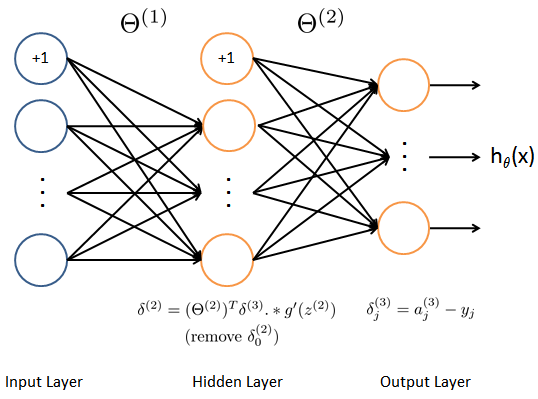
\includegraphics[width=.9\textwidth]{src/neuralNetwork2/nnb}
\caption{Освежување на вредностите во Backpropagation}
\label{fig:backpropagation}
\end{figure}

За даден тренинг примерок $(x^{(t)}, y^{(t)})$, најпрво се извршува „изминување
нанапред“ за да се добијат активациските вредности во мрежата, вклучувајќи ги и
излезните вредности на хипотезата $h_\theta(x)$. Потоа, за секој јазел $j$ во
слојот $l$, сакаме да ја пресметаме „грешката“ $\delta_j^{(l)}$ која означува
колку секој јазел во мрежата е „одговорен“ за грешките во излезот.

За излезните јазли, можеме директно да ја измериме разликата меѓу активацијата
на мрежата и вистинската вредност и да ја искористиме за да ја дефинираме
$\delta_j^{(3)}$ (слојот 3 е излезниот слој). а скриените единици,
$\delta_j^{(l)}$ го пресметуваме како тежински просек на изразите за грешка на
слојот $(l + 1)$.

Детално чекорите на backpropagation алгоритмот се следните:

\begin{enumerate}
  \item Поставете ги вредностите на влезниот слој $(a^{(1)})$ на вредностите од
  $t-$тиот тренинг примерок $x^{(t)}$. Следува feedforward (Слика
  \ref{fig:backpropagation}), за пресметување на активациите $z^{(2)}, a^{(2)},
  z^{(3)}, a^{(3)}$ за слоевите 2 и 3. Исто така треба да се додаде и изразот a + 1 за да активациските
  вектори за слоевите $a^{(1)}$ и $a^{(2)}$ исто така ја вклучуваат единицата
  за наклонетост. Во Matlab и Octave, ако 1 е вектор колона, додавање 1 е
  еквивалентно на \begin{verbatim} a_1 = [1; a_1]. \end{verbatim}
  \item За секоја излезна единица $k$ во слојот 3 (излезниот слој), пресметајте:
  \[
  	\delta_k^{(3)} = (a^{(k)} - y_k),
	\]
	каде што $y_k $ покажува дали тековниот примерок припаѓа на класата $k (y_k =
	1)$ или припаѓа на друга класа $(y_k = 0)$.
  \item За скриениот слој $l = 2$, пресметајте
   	\[
  	\delta^{(2)} = (\Theta^{(2)})^T \delta^{(3)} .* g'(z^{(2)}),
	\]
	\item Соберете го градиентот од овој примерок со користење на следната формула:
	\[
  	\Delta^{(l)} = \Delta^{(l)} + \delta^{(l + 1)}(a^{(l)})^T
	\]
	\item Пресметајте го (ненормализираниот) градиент за функцијата на чинење на
	неверонската мрежа со множење на збирот на градиентите со $\frac{1}{m}$:
	 \[
  	\frac{\partial}{\partial\Theta_{ij}^{(l)}} J(\Theta) = D_{ij}^{(l)} =
  	\frac{1}{m}\Delta_{ij}^{(l)}
	\]
	
\end{enumerate} 


\begin{figure}[htb]
\centering
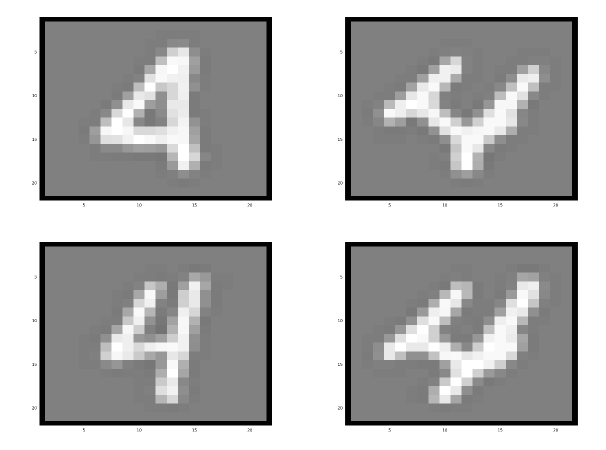
\includegraphics[width=.6\textwidth]{src/neuralNetwork1/num_4}
\caption{Четири различни прикази на бројот 4}
\label{fig:num4}
\end{figure}

\begin{figure}[htb]
\centering
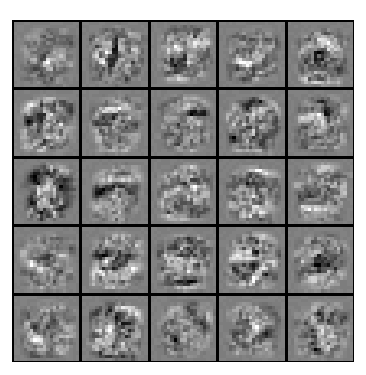
\includegraphics[width=.6\textwidth]{src/neuralNetwork2/nn_viz}
\caption{Визуелизација на тренираната невронска мрежа}
\label{fig:viz}
\end{figure}

\subsection{Примери}

На слика \ref{fig:num4} се прикажани четири различни примериоци на бројот 4 и во
сите случаи алгоритмот точно ја предвидува прикажаната бројка. На слика
\ref{fig:viz} е прикажана визуелизација на тренираната невронска мрежа.





